\documentclass[11pt,letterpaper]{article}

% Load some basic packages that are useful to have
% and that should be part of any LaTeX installation.
%
% be able to include figures
\usepackage{graphicx}
% get nice colors
\usepackage{xcolor}

% change default font to Palatino (looks nicer!)
\usepackage[latin1]{inputenc}
\usepackage{mathpazo}
\usepackage[T1]{fontenc}
% load some useful math symbols/fonts
\usepackage{latexsym,amsfonts,amsmath,amssymb}

% comfort package to easily set margins
\usepackage[top=1in, bottom=1in, left=1in, right=1in]{geometry}

% control some spacings
%
% spacing after a paragraph
\setlength{\parskip}{.15cm}
% indentation at the top of a new paragraph
\setlength{\parindent}{0.0cm}
\usepackage{dtklogos}


\begin{document}

\begin{center}
\Large
Ay190 -- Worksheet 1\\
Scott Barenfeld\\
Date: \today
\end{center}

\section{Problem 1}
I successfully installed VirtualBox and ran the 190 virtual machine.

%See figure~\ref{fig:simpleplot2} for an example!

%{\bf This is text in bold font.}

%\emph{This is text in italic font.}

%{\it This also produces italic font.}

%{\color{red} This is text in red!}

%\subsection{This is a Subsection}

%\subsubsection{This is a Subsubsection}

\section{Problem 2}
I set up my repository, emailed the name, and made a ws1 subdirectory.

\section{Problem 3}
\subsection{Part c}
I modified \texttt{simpleplot.py} to make a pdf file.  I also modified 
\texttt{simpleplot2.py} to add a third curve (see Fig. \ref{fig:simpleplot2}).

\begin{figure}[bth]
\centering
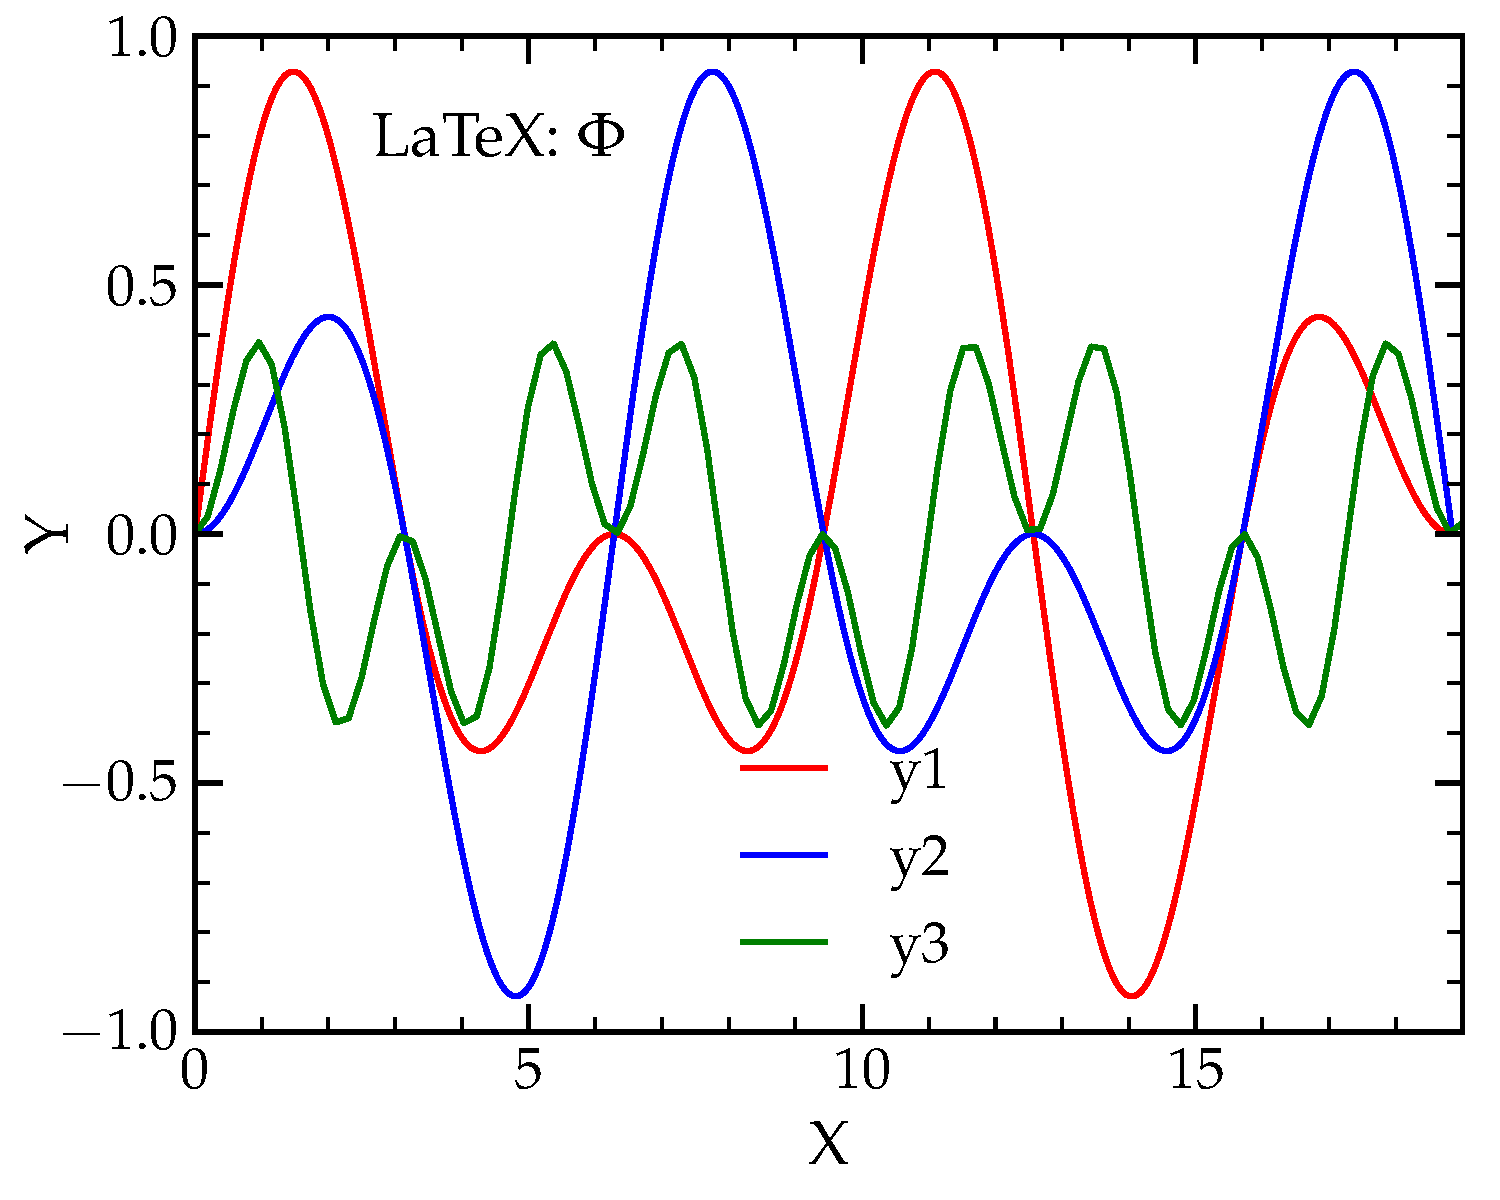
\includegraphics[width=0.5\textwidth]{simpleplot2.pdf}
\caption{This is a figure.}
\label{fig:simpleplot2}
\end{figure}

\subsection{Pard d}
I compiled the template \LaTeX\, document and added a reference to the \BibTeX\, file.  
I wrote a \texttt{Makefile} to compile the \BibTeX\, example with one command.

\end{document}
Anything that comes after \end{document} is completely
ignored by LaTeX.
